\documentclass{article}

\usepackage{tikz,amssymb,amsmath,color,alltt}
\usepackage{graphics}
\usetikzlibrary{arrows,snakes,backgrounds}
\usetikzlibrary{shapes,shapes.multipart}
\usepackage{hyperref}
\def\btr{\blacktriangleright}
\def\vtr{\vartriangleright}
\def\cS{{\mathcal S}}

\def\nil{\mbox{\sc Nil}}
\def\ptn{\mbox{\tt pointer\_to\_node}}
\def\pp{\mbox{\tt ->}}
\def\red{\mbox{\sc Red}}
\def\black{\mbox{\sc Black}}

\newcommand\comment[1]{}
\newcommand\blu[1]{{\color{blue} {#1}}}
\newcommand\grn[1]{{\color{green!50!black} #1}}
\def\lra{\leftrightarrow}
%%
\newcommand\sra[1]{\stackrel{#1}{\rightsquigarrow}}

\newcommand\pair[1]{\langle{#1}\rangle}
\def\la{\leftarrow}
\def\pl{\textsc{Prolog}}
\def\Ra{\Rightarrow}
\def\cH{\mathcal{H}}

\title{{\small\sc Advanced Data Structures}\\
Lab 1 -- Answers}
\date{}
\begin{document}
\maketitle
\subsection*{Labwork 1 -- reversing a linked list in linear time}
\begin{verbatim}

#include <iostream>
using namespace std;

struct Node {
  int key;
  Node *sibling;
  Node(int k, Node* s) { key = k; sibling = s; }
};

Node* reverseList(Node* ptr) {
  if (ptr == NULL || ptr->sibling == NULL) return ptr;
  Node* next    = ptr->sibling;
  Node* result  = reverseList(next);
  next->sibling = ptr;
  ptr->sibling  = NULL;
  return result;
}

void showList(Node* ptr) {
  Node* crt = ptr;
  while (crt != NULL) {
    cout << crt->key << " ";
    crt = crt->sibling;
  }
}

Node* readList(int m) {
    Node* ptr = NULL;
    int k;
    for (int i=0;i<m;i++) { cin >> k; ptr = new Node(k,ptr); }
    return ptr;
}

int main() {
  Node* crt = readList(10);
  cout << "List: ";
  showList(crt);
  cout << "\nReversed list: ";
  showList(reverseList(crt));
  return 0;
}
\end{verbatim}

\subsection*{Labwork 2 - binomial heaps}
\begin{verbatim}
Node* reverseList(Node* l) {
  if (l == NULL || l->sibling == NULL) return l;
  Node* next    = l->sibling;
  Node* result  = reverseList(next);
  next->sibling = l;
  l->sibling    = NULL;
  return result;
}

Node* findMinRoot(Node* n) {
  if (n == NULL) return n;
     Node* minNode = n;
   Node* crt = n;
   while (crt->sibling != NULL) {
     crt = crt->sibling;
     if (crt->key < minNode->key) minNode = crt;
   }
   return minNode;
}
\end{verbatim}
\subsection*{Exercises}
 \begin{enumerate}
\item[1.(a)]  \verb|x->sibling->degree < x->degree|
\item[1.(b)]  \verb|x->sibling->degree > x->degree|
\item[2.] 
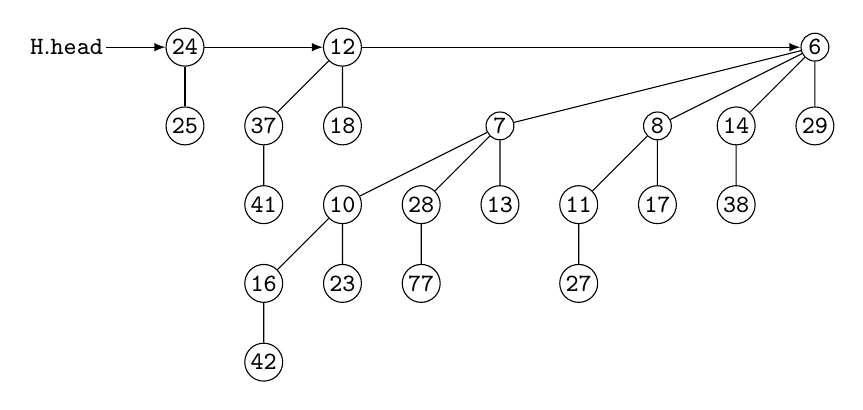
\begin{tikzpicture}[>=latex,inner sep=1pt,baseline=5.3em]
\node[left] (H) at (0,2) {\small $\tt H.head$};
\node[circle,draw] (n1) at (1,2) {\small\tt  24};
\node[circle,draw] (pic) at (1,1) {\small\tt  25};
\draw (n1) -- (pic);
%
\node[circle,draw] (n2) at (3,2) {\small\tt  12};
\node[circle,draw] (u1) at (2,1) {\small\tt  37};
\node[circle,draw] (u2) at (3,1) {\small\tt  18};
\node[circle,draw] (v0) at (2,0) {\small\tt  41};
\draw (v0) -- (u1) -- (n2) -- (u2);
\node[circle,draw] (n3) at (9,2) {\small\tt  6};
\node[circle,draw] (u3) at (5,1) {\small\tt 7};
\node[circle,draw] (x1) at (3,0) {\small\tt 10};
\node[circle,draw] (x2) at (4,0) {\small\tt 28};
\node[circle,draw] (x3) at (5,0) {\small\tt 13};
\node[circle,draw] (y1) at (2,-1) {\small\tt 16};
\node[circle,draw] (y2) at (3,-1) {\small\tt 23};
\node[circle,draw] (y3) at (4,-1) {\small\tt 77};
\node[circle,draw] (x) at (2,-2) {\small\tt  42};
\draw (x1) -- (u3) -- (x2) (x3) --(u3) (y3) -- (x2)  (x)--(y1) -- (x1) -- (y2);
\node[circle,draw] (u4) at (7,1) {\small\tt 8};
\node[circle,draw] (uu4) at (7,0) {\small\tt 17};
\node[circle,draw] (uu3) at (6,0) {\small\tt 11};
\node[circle,draw] (uuu3) at (6,-1) {\small\tt 27};
\node[circle,draw] (u5) at (8,1) {\small\tt 14};
\node[circle,draw] (uu5) at (8,0) {\small\tt 38};
\draw (uu5) -- (u5) (uu4) -- (u4) -- (uu3) -- (uuu3);
\node[circle,draw] (u6) at (9,1) {\small\tt 29};
\draw[->] (H) -- (n1); \draw[->] (n1) -- (n2); \draw[->] (n2) -- (n3);
\draw (u3) -- (n3) -- (u4); \draw (u5) -- (n3) -- (u6);
\end{tikzpicture}
\item [3.]Removing node with key 28 from the binomial heap
\begin{center}
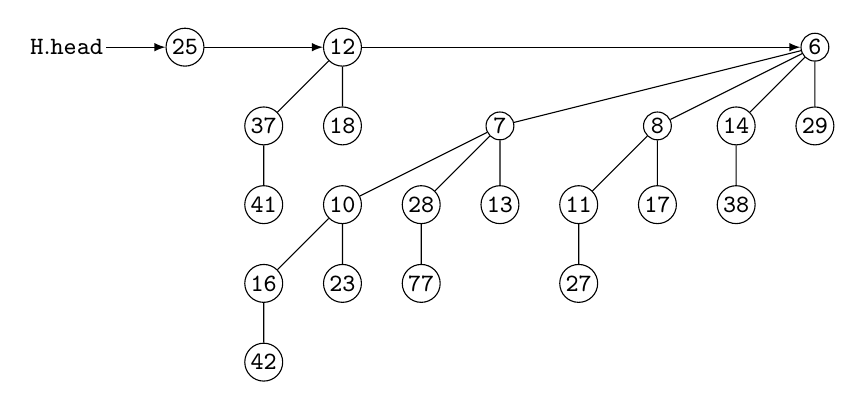
\begin{tikzpicture}[>=latex,inner sep=1pt]
\node[left] (H) at (0,2) {\small $\tt H.head$};
\node[circle,draw] (n1) at (1,2) {\small\tt  25};
\node[circle,draw] (n2) at (3,2) {\small\tt  12};
\node[circle,draw] (u1) at (2,1) {\small\tt  37};
\node[circle,draw] (u2) at (3,1) {\small\tt  18};
\node[circle,draw] (v0) at (2,0) {\small\tt  41};
\draw (v0) -- (u1) -- (n2) -- (u2);
\node[circle,draw] (n3) at (9,2) {\small\tt  6};
\node[circle,draw] (u3) at (5,1) {\small\tt 7};
\node[circle,draw] (x1) at (3,0) {\small\tt 10};
\node[circle,draw] (x2) at (4,0) {\small\tt 28};
\node[circle,draw] (x3) at (5,0) {\small\tt 13};
\node[circle,draw] (y1) at (2,-1) {\small\tt 16};
\node[circle,draw] (y2) at (3,-1) {\small\tt 23};
\node[circle,draw] (y3) at (4,-1) {\small\tt 77};
\node[circle,draw] (x) at (2,-2) {\small\tt  42};
\draw (x1) -- (u3) -- (x2) (x3) --(u3) (y3) -- (x2)  (x)--(y1) -- (x1) -- (y2);
\node[circle,draw] (u4) at (7,1) {\small\tt 8};
\node[circle,draw] (uu4) at (7,0) {\small\tt 17};
\node[circle,draw] (uu3) at (6,0) {\small\tt 11};
\node[circle,draw] (uuu3) at (6,-1) {\small\tt 27};
\node[circle,draw] (u5) at (8,1) {\small\tt 14};
\node[circle,draw] (uu5) at (8,0) {\small\tt 38};
\draw (uu5) -- (u5) (uu4) -- (u4) -- (uu3) -- (uuu3);
\node[circle,draw] (u6) at (9,1) {\small\tt 29};
\draw[->] (H) -- (n1); \draw[->] (n1) -- (n2); \draw[->] (n2) -- (n3);
\draw (u3) -- (n3) -- (u4); \draw (u5) -- (n3) -- (u6);
\end{tikzpicture}
\end{center}
proceeds as follows:
\begin{enumerate}
\item First, we replace 28 with $-\infty$ and ``bubble-up'' the node $-\infty$ until it becomes node on the root list. The binomial heap changes into
\begin{center}
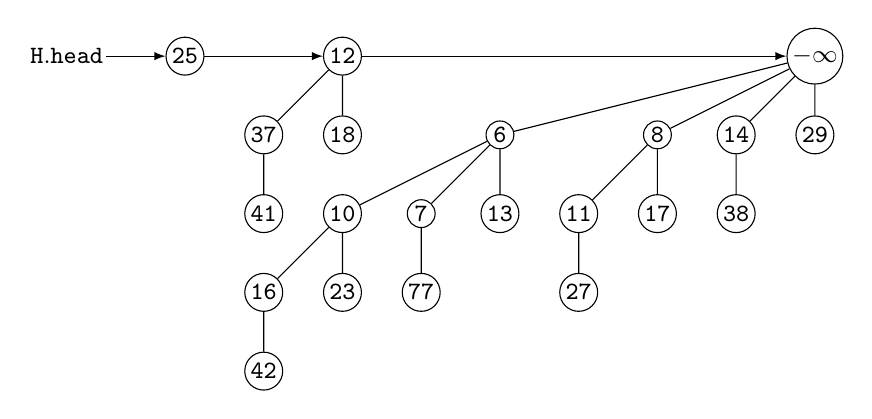
\begin{tikzpicture}[>=latex,inner sep=1pt]
\node[left] (H) at (0,2) {\small $\tt H.head$};
\node[circle,draw] (n1) at (1,2) {\small\tt  25};
\node[circle,draw] (n2) at (3,2) {\small\tt  12};
\node[circle,draw] (u1) at (2,1) {\small\tt  37};
\node[circle,draw] (u2) at (3,1) {\small\tt  18};
\node[circle,draw] (v0) at (2,0) {\small\tt  41};
\draw (v0) -- (u1) -- (n2) -- (u2);
\node[circle,draw] (n3) at (9,2) {\small $-\infty$};
\node[circle,draw] (u3) at (5,1) {\small\tt 6};
\node[circle,draw] (x1) at (3,0) {\small\tt 10};
\node[circle,draw] (x2) at (4,0) {\small \tt 7};
\node[circle,draw] (x3) at (5,0) {\small\tt 13};
\node[circle,draw] (y1) at (2,-1) {\small\tt 16};
\node[circle,draw] (y2) at (3,-1) {\small\tt 23};
\node[circle,draw] (y3) at (4,-1) {\small\tt 77};
\node[circle,draw] (x) at (2,-2) {\small\tt  42};
\draw (x1) -- (u3) -- (x2) (x3) --(u3) (y3) -- (x2)  (x)--(y1) -- (x1) -- (y2);
\node[circle,draw] (u4) at (7,1) {\small\tt 8};
\node[circle,draw] (uu4) at (7,0) {\small\tt 17};
\node[circle,draw] (uu3) at (6,0) {\small\tt 11};
\node[circle,draw] (uuu3) at (6,-1) {\small\tt 27};
\node[circle,draw] (u5) at (8,1) {\small\tt 14};
\node[circle,draw] (uu5) at (8,0) {\small\tt 38};
\draw (uu5) -- (u5) (uu4) -- (u4) -- (uu3) -- (uuu3);
\node[circle,draw] (u6) at (9,1) {\small\tt 29};
\draw[->] (H) -- (n1); \draw[->] (n1) -- (n2); \draw[->] (n2) -- (n3);
\draw (u3) -- (n3) -- (u4); \draw (u5) -- (n3) -- (u6);
\end{tikzpicture}
\end{center}
\item We remove the node with minimum key $-\infty$ from this binomial heap.
This works as follows:
\begin{itemize}
\item We break $H$ into two binomial heaps: $\tt H_1$ is $H$ without the tree with root $-\infty$; and $\tt H_2$ is the binomial heap consisting of the subtrees of $-\infty$ in reverse order:
\begin{center}
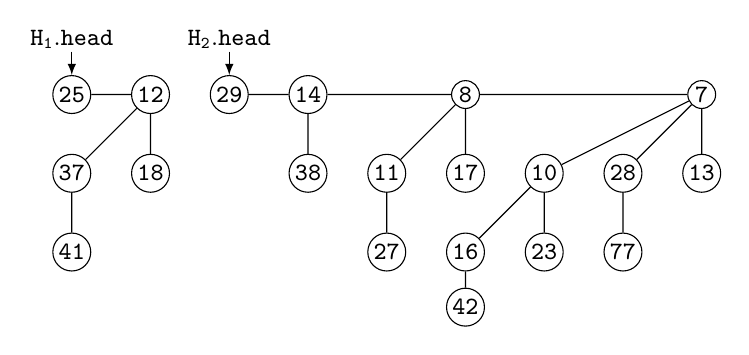
\begin{tikzpicture}[>=latex,inner sep=1pt]
\node (H1) at (0,2.7) {\small $\tt H_1.head$};
\node (H2) at (2,2.7) {\small $\tt H_2.head$};
\node[circle,draw] (n1) at (0,2) {\small\tt  25};
\node[circle,draw] (n2) at (1,2) {\small\tt  12};
\node[circle,draw] (u1) at (0,1) {\small\tt  37};
\node[circle,draw] (u2) at (1,1) {\small\tt  18};
\node[circle,draw] (v0) at (0,0) {\small\tt  41};
%
\node[circle,draw] (a0) at (2,2) {\small\tt 29};
\node[circle,draw] (a1) at (3,2) {\small\tt 14};
\node[circle,draw] (b1) at (3,1) {\small\tt 38};
\node[circle,draw] (a2) at (5,2) {\small\tt 8};
\node[circle,draw] (b2) at (4,1) {\small\tt 11};
\node[circle,draw] (c1) at (4,0) {\small\tt 27};
\node[circle,draw] (b3) at (5,1) {\small\tt 17};
%
\node[circle,draw] (a3) at (8,2) {\small\tt 7};
%
\node[circle,draw] (b4) at (6,1) {\small\tt 10};
\node[circle,draw] (c3) at (5,0) {\small\tt 16};
\node[circle,draw] (d1) at (5,-.7) {\small\tt 42};

\node[circle,draw] (c4) at (6,0) {\small\tt 23};

\node[circle,draw] (b5) at (7,1) {\small\tt 28};
\node[circle,draw] (c2) at (7,0) {\small\tt 77};
\node[circle,draw] (b6) at (8,1) {\small\tt 13};
%
\draw[->] (H1) -- (n1);
\draw[->] (H2) -- (a0) ;
\draw (a0) -- (a1) -- (a2) -- (a3) (a1) -- (b1) (c1) -- (b2) -- (a2) -- (b3) (b4) -- (a3) -- (b5) -- (c2) (a3) -- (b6);
\draw (n1) -- (n2) -- (u2) (n2) -- (u1) -- (v0) (d1) -- (c3) -- (b4) -- (c4);
\end{tikzpicture}
\end{center}
\item We merge the binomial heaps $\tt H_1$ and $\tt H_2$ as lists of trees sorted in increasing order of their degree $\Ra$ the  lists of binomial trees
\begin{center}
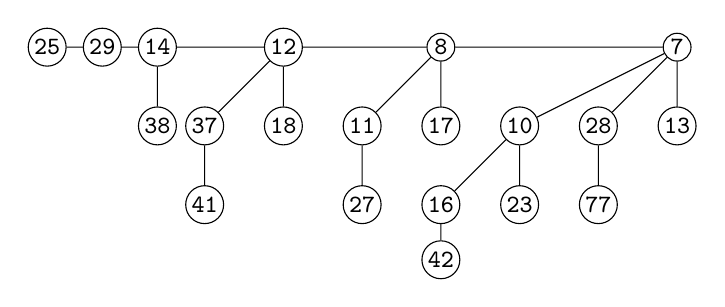
\begin{tikzpicture}[>=latex,inner sep=1pt]
\node[circle,draw] (n1) at (-2,2) {\small\tt  25};
\node[circle,draw] (a0) at (-1.3,2) {\small\tt  29};
\node[circle,draw] (a1) at (-.6,2) {\small\tt 14};
\node[circle,draw] (b1) at (-.6,1) {\small\tt 38};
\node[circle,draw] (n2) at (1,2) {\small\tt  12};
\node[circle,draw] (u1) at (0,1) {\small\tt  37};
\node[circle,draw] (u2) at (1,1) {\small\tt  18};
\node[circle,draw] (v0) at (0,0) {\small\tt  41};
%
\node[circle,draw] (a2) at (3,2) {\small\tt 8};
\node[circle,draw] (b2) at (2,1) {\small\tt 11};
\node[circle,draw] (c1) at (2,0) {\small\tt 27};
\node[circle,draw] (b3) at (3,1) {\small\tt 17};
%%
\node[circle,draw] (a3) at (6,2) {\small\tt 7};
%
\node[circle,draw] (b4) at (4,1) {\small\tt 10};
\node[circle,draw] (c3) at (3,0) {\small\tt 16};
\node[circle,draw] (d1) at (3,-.7) {\small\tt 42};

\node[circle,draw] (c4) at (4,0) {\small\tt 23};

\node[circle,draw] (b5) at (5,1) {\small\tt 28};
\node[circle,draw] (c2) at (5,0) {\small\tt 77};
\node[circle,draw] (b6) at (6,1) {\small\tt 13};
%%
\draw (n1) -- (a0) -- (a1)  -- (n2) -- (u2) (a3) -- (a2) -- (n2) -- (u1) -- (v0) 
 (c1) -- (b2) -- (a2) -- (b3) (a1) -- (b1)
 (b4) -- (a3) -- (b5) -- (c2) (a3) -- (b6) (d1) -- (c3) -- (b4) -- (c4);
\end{tikzpicture}
\end{center}
\item The previous list is not a binomial heap because it contains trees with same degree. We transform it into a binomial heap by combining binomial trees with same degree (see lecture notes). 
\end{itemize}
In the end we obtain the binomial heap $H'$ depicted below:
\begin{center}
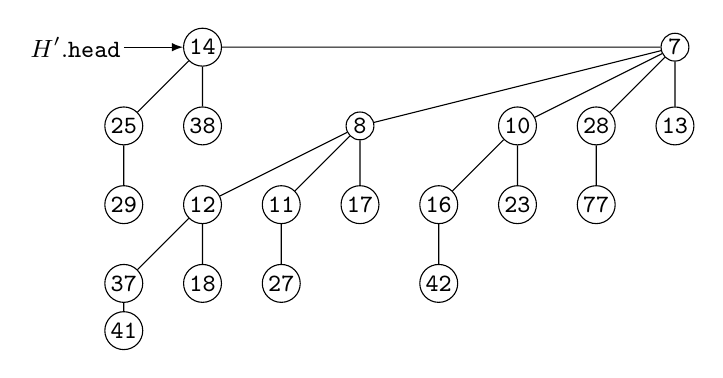
\begin{tikzpicture}[>=latex,inner sep=1pt]
\node[left] (zz) at (0,2) {\small $H'{\tt .head}$};
\node[circle,draw] (n1) at (0,1) {\small\tt  25};
\node[circle,draw] (a0) at (0,0) {\small\tt  29};
\node[circle,draw] (a1) at (1,2) {\small\tt 14};
\node[circle,draw] (b1) at (1,1) {\small\tt 38};
\node[circle,draw] (n2) at (1,0) {\small\tt  12};
\node[circle,draw] (u1) at (0,-1) {\small\tt  37};
\node[circle,draw] (u2) at (1,-1) {\small\tt  18};
\node[circle,draw] (v0) at (0,-1.6) {\small\tt  41};
%
\node[circle,draw] (a2) at (3,1) {\small\tt 8};
\node[circle,draw] (b2) at (2,0) {\small\tt 11};
\node[circle,draw] (c1) at (2,-1) {\small\tt 27};
\node[circle,draw] (b3) at (3,0) {\small\tt 17};
%%
\node[circle,draw] (a3) at (7,2) {\small\tt 7};
%
\node[circle,draw] (b4) at (5,1) {\small\tt 10};
\node[circle,draw] (c3) at (4,0) {\small\tt 16};
\node[circle,draw] (d1) at (4,-1) {\small\tt 42};

\node[circle,draw] (c4) at (5,0) {\small\tt 23};

\node[circle,draw] (b5) at (6,1) {\small\tt 28};
\node[circle,draw] (c2) at (6,0) {\small\tt 77};
\node[circle,draw] (b6) at (7,1) {\small\tt 13};
%%
\draw[->] (zz) -- (a1);
\draw (n1) -- (a0)  (n1) -- (a1)  -- (a3) (n2) -- (u2) (a3) -- (a2) -- (n2) -- (u1) -- (v0) 
 (c1) -- (b2) -- (a2) -- (b3) (a1) -- (b1)
 (b4) -- (a3) -- (b5) -- (c2) (a3) -- (b6) (d1) -- (c3) -- (b4) -- (c4);
\end{tikzpicture}
\end{center}
\end{enumerate}
\item[4.] Increasing the value of a key implies the need to push down the node with increased key, by swapping the node with the child with minimum key. The pseudocode of this operation is
\begin{tabbing}
increaseKey(H\(,x,k\))\\
1 {\bf if} \=$k\leq x\mbox{\tt->}key$\\
2\>{\bf error} ``new key is not greater than current key''\\
3 $x\mbox{\tt->}key:=k$\\
4 $y:=x$\\
5 {\bf while} \=$y\mbox{\tt->}child\neq\mbox{\tt NIL}$\\
6\>$z:=$child of $y$ with minimum key among children of $y$\\
7\>{\bf if} \=$y\mbox{\tt->}key>z\mbox{\tt->}key$\\
8\>\>exchange $y\mbox{\tt->}key\leftrightarrow z\mbox{\tt->}key$\\
9\>\> if $y$ and $z$ have satellite fields, exchange them, too\\
10\>\>$y:=z$\\
11\>{\bf else} {\tt break}\\

\end{tabbing}
\begin{enumerate}
\item 
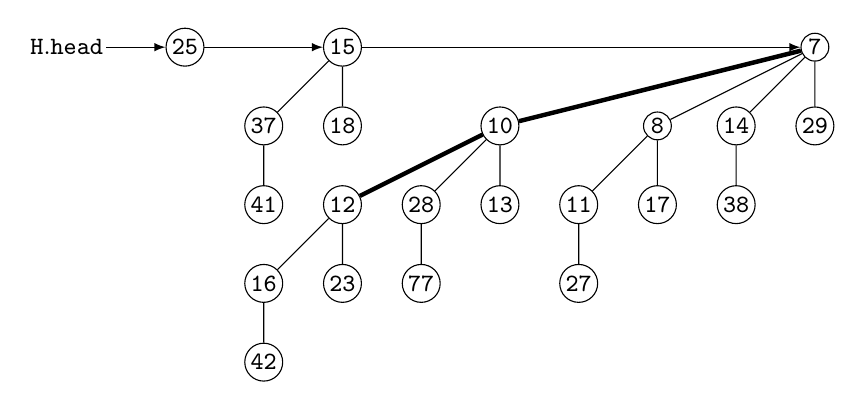
\begin{tikzpicture}[>=latex,inner sep=1pt,baseline=5.3em]
\node[left] (H) at (0,2) {\small $\tt H.head$};
\node[circle,draw] (n1) at (1,2) {\small\tt  25};
\node[circle,draw] (n2) at (3,2) {\small\tt  15};
\node[circle,draw] (u1) at (2,1) {\small\tt  37};
\node[circle,draw] (u2) at (3,1) {\small\tt  18};
\node[circle,draw] (v0) at (2,0) {\small\tt  41};
\draw (v0) -- (u1) -- (n2) -- (u2);
\node[circle,draw] (n3) at (9,2) {\small\tt  7};
%\node[right] at (9.3,2) {\small $x$};
\node[circle,draw] (u3) at (5,1) {\small\tt 10};
\node[circle,draw] (x1) at (3,0) {\small\tt 12};
\node[circle,draw] (x2) at (4,0) {\small\tt 28};
\node[circle,draw] (x3) at (5,0) {\small\tt 13};
\node[circle,draw] (y1) at (2,-1) {\small\tt 16};
\node[circle,draw] (y2) at (3,-1) {\small\tt 23};
\node[circle,draw] (y3) at (4,-1) {\small\tt 77};
\node[circle,draw] (x) at (2,-2) {\small\tt  42};
\draw (x1) -- (u3) -- (x2) (x3) --(u3) (y3) -- (x2)  (x)--(y1) -- (x1) -- (y2);
\node[circle,draw] (u4) at (7,1) {\small\tt 8};
\node[circle,draw] (uu4) at (7,0) {\small\tt 17};
\node[circle,draw] (uu3) at (6,0) {\small\tt 11};s
\node[circle,draw] (uuu3) at (6,-1) {\small\tt 27};
\node[circle,draw] (u5) at (8,1) {\small\tt 14};
\node[circle,draw] (uu5) at (8,0) {\small\tt 38};
\draw (uu5) -- (u5) (uu4) -- (u4) -- (uu3) -- (uuu3);
\node[circle,draw] (u6) at (9,1) {\small\tt 29};
\draw[->] (H) -- (n1); \draw[->] (n1) -- (n2); \draw[->] (n2) -- (n3);
\draw (u3) -- (n3) -- (u4); \draw (u5) -- (n3) -- (u6);
\draw[ultra thick] (n3) -- (u3) -- (x1);
\end{tikzpicture}
\item The worst happens when $H$ has only one binomial tree with $n=2^m$ nodes, the longest branch from the root is is $x_0{-}x_1{-}\ldots{-}x_m$ such that every node $x_i$ has smallest key in the list of children of $x_{i-1}$, and $k>x_m\mbox{\tt->}key$. In this case, we must perform 
 $m$ node exchanges, and $(m-1)(m-2)/2$ key comparisons to find the child nodes with minimum key.
 The worst runtime complexity ia $O(\log^2(m))$.
\item $16=2^4\Ra$ we can have the worst case for
\begin{center}
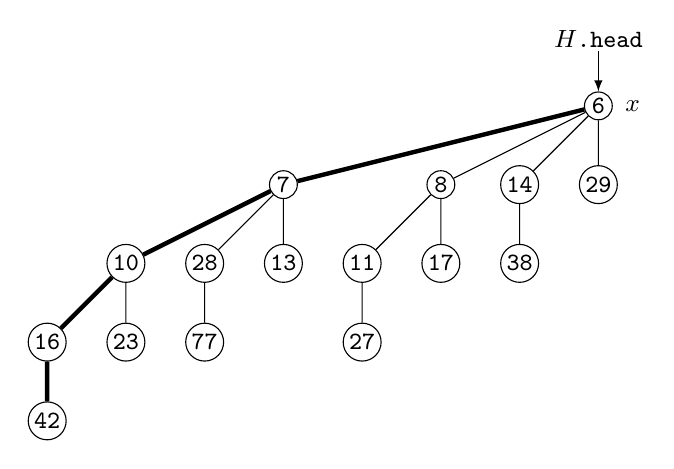
\begin{tikzpicture}[>=latex,inner sep=1pt]
\node[above] (n2) at (9,2.7) {\small $H$\tt.head};
\node[circle,draw] (n3) at (9,2) {\small\tt  6};
\node[right] at (9.3,2) {\small $x$};
\node[circle,draw] (u3) at (5,1) {\small\tt 7};
\node[circle,draw] (x1) at (3,0) {\small\tt 10};
\node[circle,draw] (x2) at (4,0) {\small\tt 28};
\node[circle,draw] (x3) at (5,0) {\small\tt 13};
\node[circle,draw] (y1) at (2,-1) {\small\tt 16};
\node[circle,draw] (y2) at (3,-1) {\small\tt 23};
\node[circle,draw] (y3) at (4,-1) {\small\tt 77};
\node[circle,draw] (x) at (2,-2) {\small\tt  42};
\draw (x1) -- (u3) -- (x2) (x3) --(u3) (y3) -- (x2)  (x)--(y1) -- (x1) -- (y2);
\node[circle,draw] (u4) at (7,1) {\small\tt 8};
\node[circle,draw] (uu4) at (7,0) {\small\tt 17};
\node[circle,draw] (uu3) at (6,0) {\small\tt 11};
\node[circle,draw] (uuu3) at (6,-1) {\small\tt 27};
\node[circle,draw] (u5) at (8,1) {\small\tt 14};
\node[circle,draw] (uu5) at (8,0) {\small\tt 38};
\draw (uu5) -- (u5) (uu4) -- (u4) -- (uu3) -- (uuu3);
\node[circle,draw] (u6) at (9,1) {\small\tt 29};
 \draw[->] (n2) -- (n3);
\draw (u3) -- (n3) -- (u4); \draw (u5) -- (n3) -- (u6);
\draw[ultra thick] (n3) -- (u3) -- (x1) -- (y1) -- (x);
\end{tikzpicture}
\end{center}
and we increase the key of $x$ from {\tt 6} to {\tt 43}.
\end{enumerate}
\end{enumerate}
\end{document}